XORを学習するニューラルネットワークを作成した.
リスト\ref{sampleBP.c}に示すプログラムを用いて
実行を行った.

XORの各入力に対して学習がうまくいっていることを
確認した.

また,拡張として行列演算によって前向き,後ろ向き
の計算を行うリスト\ref{newral.py}のプログラム
も作成した.
なお,リスト\ref{sampleBP.c}と同じ重みを用いて学習を
行い,結果が同じになることを確認している.
同様に学習がうまくいっていることを確認した.

学習過程の誤差の変化を図\ref{error-1}に示す.

\begin{figure}[htb]
  \centering
  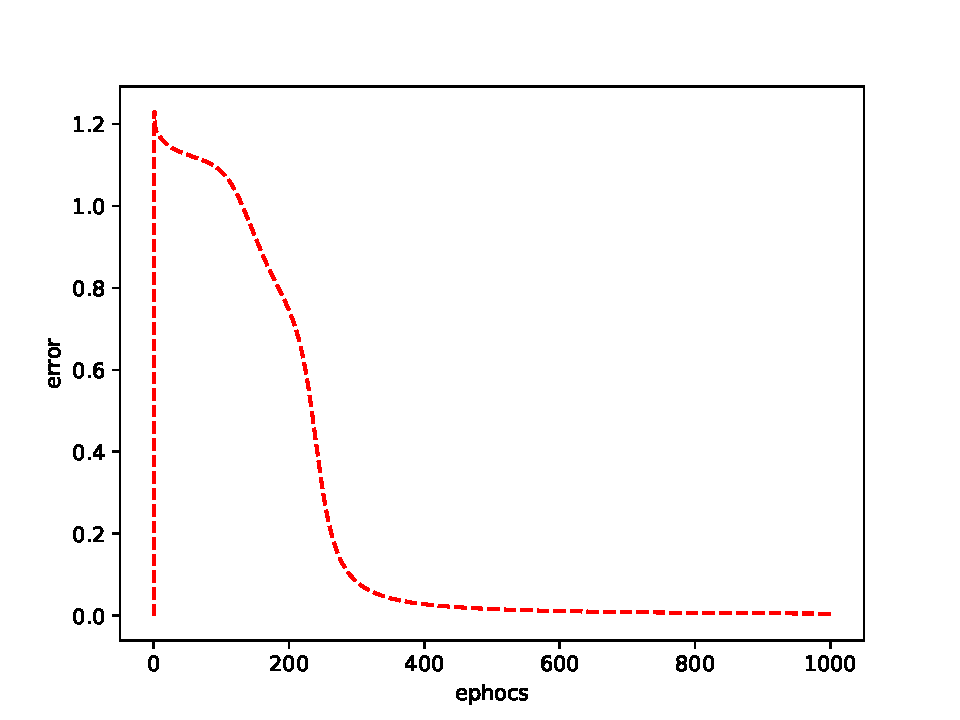
\includegraphics[scale=0.5]{img/error1.pdf}
  \caption{XOR学習時の誤差変化}
  \label{error-1}
\end{figure}
